\section{Subsistema: Perfuração e Coleta}

  \subsection{Sistema de Perfuração}
  
  Para o sistema de perfuração algumas pesquisas e discussões foram feitas para escolher um sistema que pudesse ser realizado. Foram definidas duas opções possíveis para serem comparadas e analisadas e depois decidir a que se encaixa melhor nos requisitos do projeto.

  \textbf{Opção A}: Usar uma broca para perfurar o plástico e a terra, ao completar este
  processo, um dispositivo é acionado para realizar a troca da peça broca para
  a peça sensor, o sensor de umidade é então estendido até o solo do buraco e
  coleta os dados solicitados. Após a coleta dos dados o sensor é recolhido e o
  carrinho segue em frente para mais uma perfuração.

  \textbf{Opção B}: Usar um tubo puntiforme contendo o sensor, havendo na ponta do tubo
  aberturas levemente maiores que as dimensões dos terminais do sensor. O tubo
  terá um motor para empurrá-lo até a lona e fazer o furo desejado; um servo
  motor estenderá o sensor para que ele possa fazer a medição da umidade.

  O grupo optou pela opção B pelos seguintes fatores:

  \begin{itemize}
    \item Dificuldade em elaborar um mecanismo para alternar a broca e o sensor
    conforme descrito na opção A;
    \item Relativa facilidade em perfurar o solo devido a sua baixa compactabilidade
    \item Diminuição da quantidade de atuadores necessários.
  \end{itemize}

  O motor definido para uso no sistema de perfuração também será o
  Mabachi GD - 558RC/LC 12V, tendo em vista que seu torque máximo supre as
  condições de resistência que o solo pode impor.

  Já para a extensão do sensor para o solo, será utilizado o servo motor Tower
  Pro Mg90s Metal Gear, tendo como base o torque de 2,2 Kg/cm quando operado na faixa de 6V.

% Daqui para a frente quem escreve é o PG e o Fagner {{{
\subsection{Sensoriamento: Coleta}


  % Sensor de Umidade e Temperatura (AM2302) {{{
	\subsubsection{Sensor de Umidade e Temperatura do Ar (AM2302)}

		O sensor escolhido para as medições de temperatura e umidade relativa do ar
		é o AM2302 (idêntico ao DHT22) da AOSONG que é apresentado na figura~\ref{fig:AM2302}.

		\begin{figure}[!htbp]
		\begin{center}
		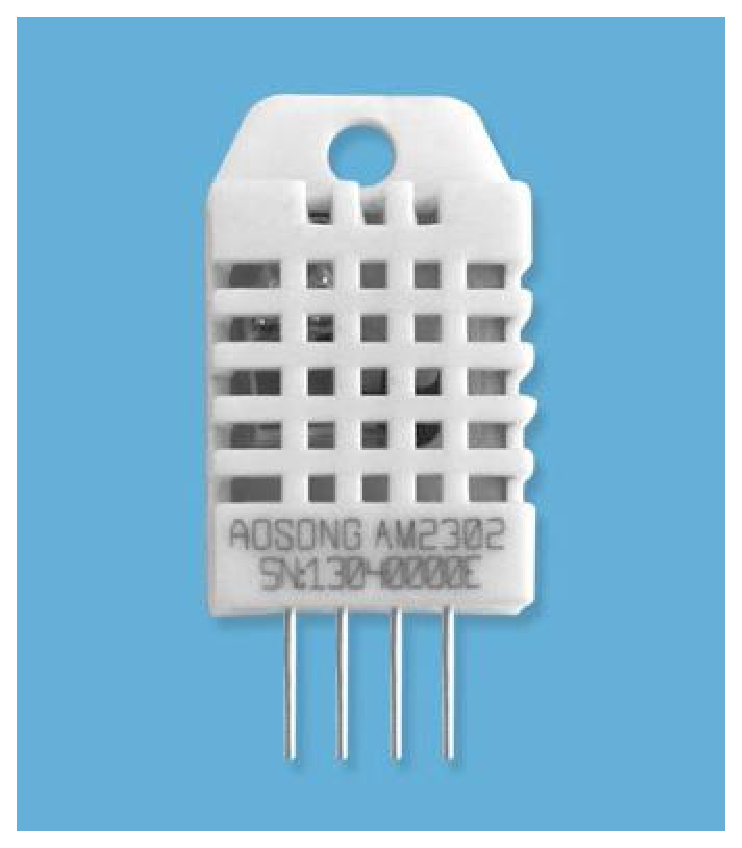
\includegraphics[width=.4\textwidth]{figuras/am2302.eps}
		\caption{\label{fig:AM2302}Sensor de umidade relativa e temperatura do ar (fonte:~\citeonline{aosong}).}
		\end{center}
		\end{figure}

		O AM2302 contém um sensor capacitivo de umidade para a medição da umidade relativa
		do ar com uma resolução de $0.1~\%\textrm{RH}$ e precisão de $\pm 2~\%\textrm{RH}$.
		Além do sensor de umidade, este módulo também contém um sensor de temperatura com
		alta precisão e alcance de $-40~\celsius$ à $80~\celsius$, resolução de $0.1~\celsius$,
		e precisão de $\pm 0.5~\celsius$~\cite{aosong}.

		O AM2302 possui um microcontrolador de 8 bits embutido com parâmetros de calibração já gravados
		que forncem medições precisas e estáveis durante um longo tempo de utilização.
		Os dados fornecidos pelos sensores são de 16 bits para temperatura e
		16 bits para umidade relativa do ar~\cite{aosong}.

		A comunicação com o dispositivo se dá por meio de um único pino (SDA, pino 2) que é
		bidirecional e são retornados 40 bits ao microcontrolador que realizou a requisição, onde
		o primeiro e o segundo bytes contém a última leitura de umidade,
		o terceiro e o quarto bytes contém a última leitura de temperatura,
		e o quinto byte contém um \textit{checksum} que é a soma dos 4 primeiros bytes
		indicando se os dados são válidos.
		O pino de alimentação é o pino 1 e ele pode ser alimentado com $3.3\textrm{V}$--$5\textrm{V}$,
		sendo $5\textrm{V}$ o recomendado. O pino 3 não é utilizado e o pino 4 é o terra.
		O tempo mínimo entre leituras consecutivas é de 2 segundos~\cite{aosong}.

	\paragraph{Implementação}

		A complexidade de implementação deste módulo é bastante reduzida
		se for utilizada uma das bibliotecas já desenvolvidas para o envio
		e leitura de dados do AM2302. Felizmente a Adafruit, uma empresa americana
		que trabalha com \textit{hardware open-source}, fornece uma biblioteca para
		a plataforma Arduino para tornar o desenvolvimento mais simples\footnote{\url{https://github.com/adafruit/DHT-sensor-library}.}.
		Portanto, foi utilizada a biblioteca \texttt{DHT.h} para os propósitos
		deste projeto.

	\paragraph{Testes}

		Os testes feitos com o módulo AM2302 foram realizados utilizando
		o \textit{hardware} apresentado na figura~\ref{fig:am2302test} (esquemático
		produzido com o auxílio da ferramenta Fritzing).

		\begin{figure}[!htbp]
		\begin{center}
		\includegraphics[width=.8\textwidth]{figuras/am2302_test.eps}
		\caption{\label{fig:am2302test}\textit{Hardware} utilizado para teste.}
		\end{center}
		\end{figure}

		Para os testes iniciais foi utilizado um Arduino Uno, onde era enviado uma requisição
		no formato de um número e então era feita a leitura e enviada pela porta serial.
		O resultado do teste é mostrado na figura~\ref{fig:am2302ardu}.

		\begin{figure}[!htbp]
		\begin{center}
		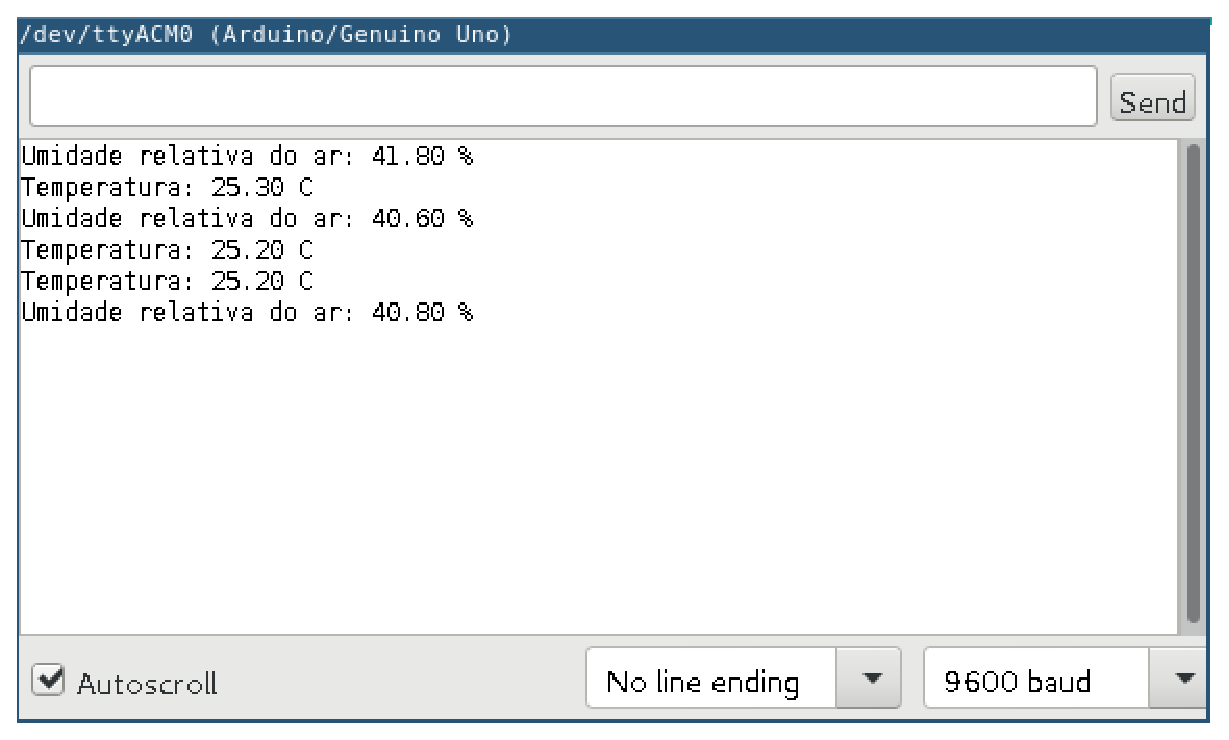
\includegraphics[width=.7\textwidth]{figuras/am2302_arduino.eps}
		\caption{\label{fig:am2302ardu}Resultado do teste da leitura dos sensores.}
		\end{center}
		\end{figure}

		Como o resultado do teste foi satisfatório é necessário realizar
		o teste de comunicação com a Raspberry Pi. Como a Raspberry possui
		um Linux embarcado e a comunicação é serial, é necessário utilizar
		as bibliotecas fornecidades pelo Linux para que a comunicação
		possa ser estabelecida, e a biblioteca mais importante neste caso
		é a \texttt{termio.h}.
		
		Os valores lidos pelo sensor se encontram no formato de ponto flutuante
		de 4 bytes (IEEE 754) e, portanto, tanto para a temperatura quanto
		para a umidade relativa do ar é necessário que o Arduino Uno envie
		4 bytes para cada. Os resultados do teste estão mostrados na figura~\ref{fig:am2302rasp}.

		\begin{figure}[!htbp]
		\begin{center}
		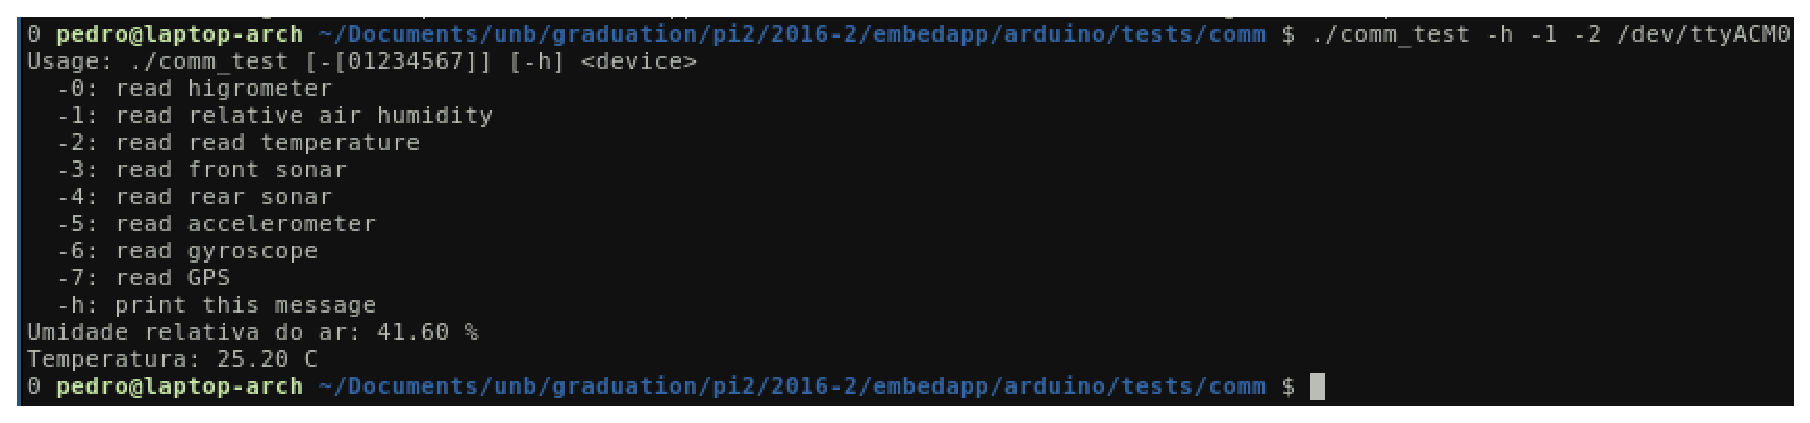
\includegraphics[width=\textwidth]{figuras/am2302_raspberry.eps}
		\caption{\label{fig:am2302rasp}Resultado do teste de comunicação com a Raspberry Pi.}
		\end{center}
		\end{figure}
  % }}}

  % Sensor de umidade do solo (FC-28) {{{
	\subsubsection{Sensor de Umidade do Solo (FC-28)}

		O sensor escolhido para a medição da umidade do solo foi o FC-28 (apresentado
		na figura~\ref{fig:fc28}),
		tanto pelo baixo custo quanto pelo simples processo de medição.
		Ele tem como princípio de medição a queda de tensão resultante da
		passagem de corrente por uma malha resistiva, que no caso seria o solo
		umedecido.

		\begin{figure}[!htbp]
		\begin{center}
		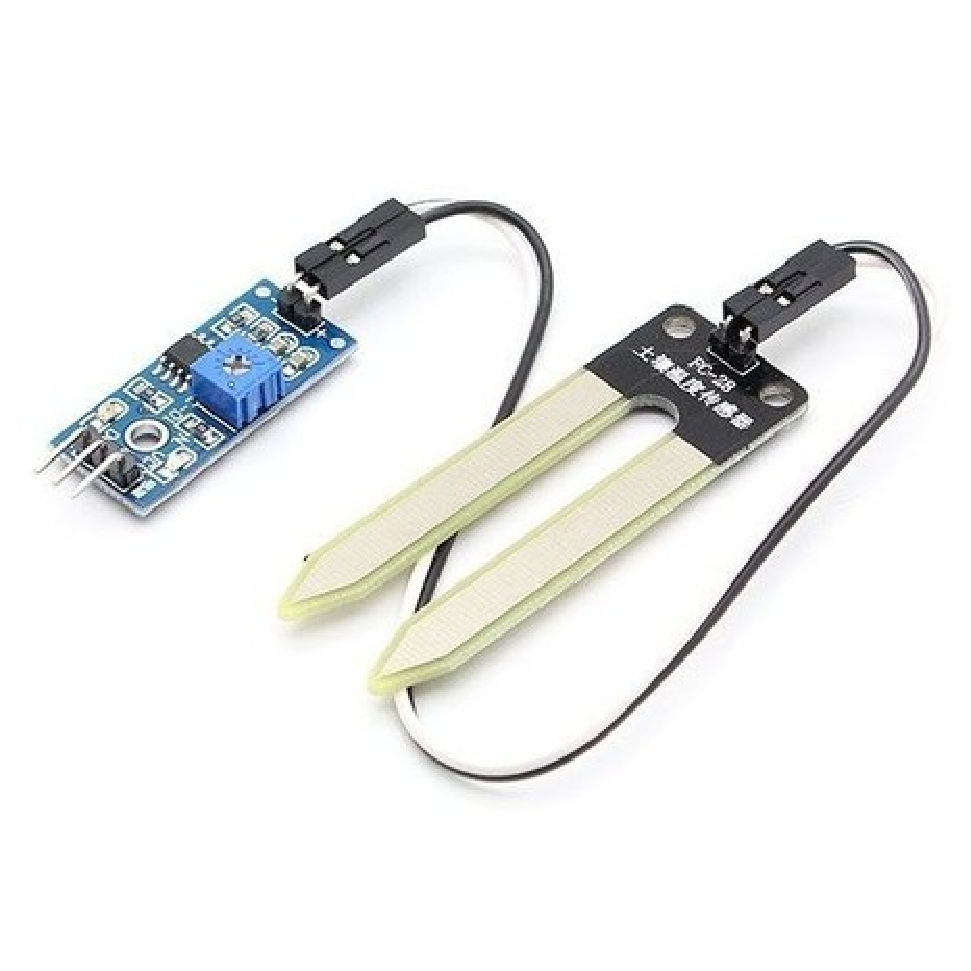
\includegraphics[width=.5\textwidth]{figuras/higrometer.eps}
		\caption{\label{fig:fc28}Sensor de umidade do solo.}
		\end{center}
		\end{figure}

		O sensor é constituído por duas linhas de eletrodos que estão
		sobrepostas a duas placas com terminações pontiagudas para facilitar a
		penetração do sensor no solo. Uma corrente é injetada em uma das linhas
		de eletrodos e é medida a queda tensão entre as linhas, que é função da
		resistência entre os eletrodos que por sua vez é função da quantidade de
		água e minerais presentes entre os eletrodos. Quando o volume de água no
		solo entre os eletrodos é baixo, ou seja, quando o solo está seco,
		a queda de tensão será maior, e quando o solo está umedecido,
		a queda de tensão é menor.

		Devido ao seu princípio de operação, este sensor mede a quantidade de
		água no solo de forma indireta, e a calibração do sensor vai de acordo
		com o que é definido como um solo seco ou úmido em um local, e portanto
		se faz necessária a calibração do equipamento em campo junto ao
		responsável pela irrigação.

		% Rotina de calibração (Fagner, 2016) {{{
		Antes do processo de calibração faz-se necessário saber sobre o processo de obtenção
		da umidade real do solo em que é preciso seguir os seguintes passos:

		\begin{itemize}
			\item Pegar uma amostra de solo do terreno colocando em um cilindro com um volume conhecido.
			\item Secar a amostra de solo com auxílio de um microondas na faixa entre 60\% a 80\% de potência.
			\item Esperar o tempo de 240 segundos ou 4 minutos exatos para estabilização da massa do solo.
			\item Pesar a amostra de solo seco guardando o valor do peso.
			\item Umedecer a amostra de solo seco.
			\item Pesar a amostra umedecida guardando o valor do peso.
			\item Calcular a umidade volumétrica com os dados do peso do solo seco, peso do solo úmido e volume do cilindro.
		\end{itemize}

		Para a secagem da amostra o procedimento padrão adotado é o uso de uma estufa de
		secagem entre $105~\celsius$ e $115~\celsius$ durante 24 horas para completa secagem da
		amostra do solo. No entanto, o método utilizando estufa é demorado para apenas
		obtenção dos dados e existe outro método que se utiliza de um microondas para
		secagem da amostra. Esse método já foi testado em experiências e comprovadamente
		funciona tão bem quanto o método de estufa de acordo com \citeonline{tavares2008uso}.

		Também é possível a partir desse procedimento, obter o valor da umidade gravimétrica
		que também pode ser usado para calibração do sensor.

		Para a necessária calibração do sensor de umidade deve-se seguir os seguintes procedimentos:

		\begin{itemize}
			\item Pegar uma amostra do solo com peso aproximado de 100 gramas.
			\item Fazer a secagem desta amostra com auxílio do microondas com potência entre 60\% a 80\%.
			\item Esperar o tempo de 240 segundos ou 4 minutos exatos para estabilização da massa do solo.
			\item Pesar a amostra de solo seco e verificar se o mesmo está com 100 gramas.
			\item Caso dê um valor acima, retirar o excesso até atingir o valor de 100 gramas,
				caso não atinja esse valor, será necessário completar a amostra e repetir o processo de secagem.
			\item Pegar uma amostra de água destilada com peso de 5 gramas e umedecer a amostra.
			\item Misturar bem a amostra até obter uma amostra homogênea.
			\item Realizar a medição dessa amostra com o sensor de umidade e obter o valor.
			\item Os valores dos pesos do solo e da água passados são intencionais, pois com
				estes valores, dará um valor de umidade gravimétrica de 5\%.
			\item O valor obtido da medida do sensor com o valor da umidade gravimétrica a
				5\% indicará que para esta umidade gravimétrica o valor da medida do sensor é equivalente.
			\item Repetir esse procedimento para amostra de solo com 10\%, 15\%, 20\%, 25\%,
				30\%, 40\%, 50\% e 60\%, sendo estas porcentagens equivalentes ao valor do peso
				da água, e comparar os valores da umidade gravimétrica com os valores de medição do sensor.
		\end{itemize}

		Dessa forma saberemos os valores equivalentes a essas porcentagens e o sensor
		estará calibrado, endoçando que para um dado valor de medida de umidade irá
		equivaler ao valor da porcentagem de umidade gravimétrica do solo.
		% }}}

		\paragraph{Implementação}

			

		\paragraph{Testes}

			
% }}}

  % Módulo de controle (Arduino Mega2560) {{{
  \subsubsection{Módulo de Controle (Arduino Mega2560)}

  Para o controle do sistema escolheu-se a placa Arduino Mega2560.
  O Mega2560 é uma placa de microcontrolador baseado no ATmega2560 .
  Ele tem 54 pinos digitais de Entrada e saída, 16 entradas analógicas,
  4 UARTs, uma conexão USB , dentre outros. Ele contém tudo o necessário
  para dar suporte ao microcontrolador. A figura~\ref{fig:arduino} apresenta a placa
  Arduino Mega2560.

  \begin{figure}[!htbp]
  \begin{center}
  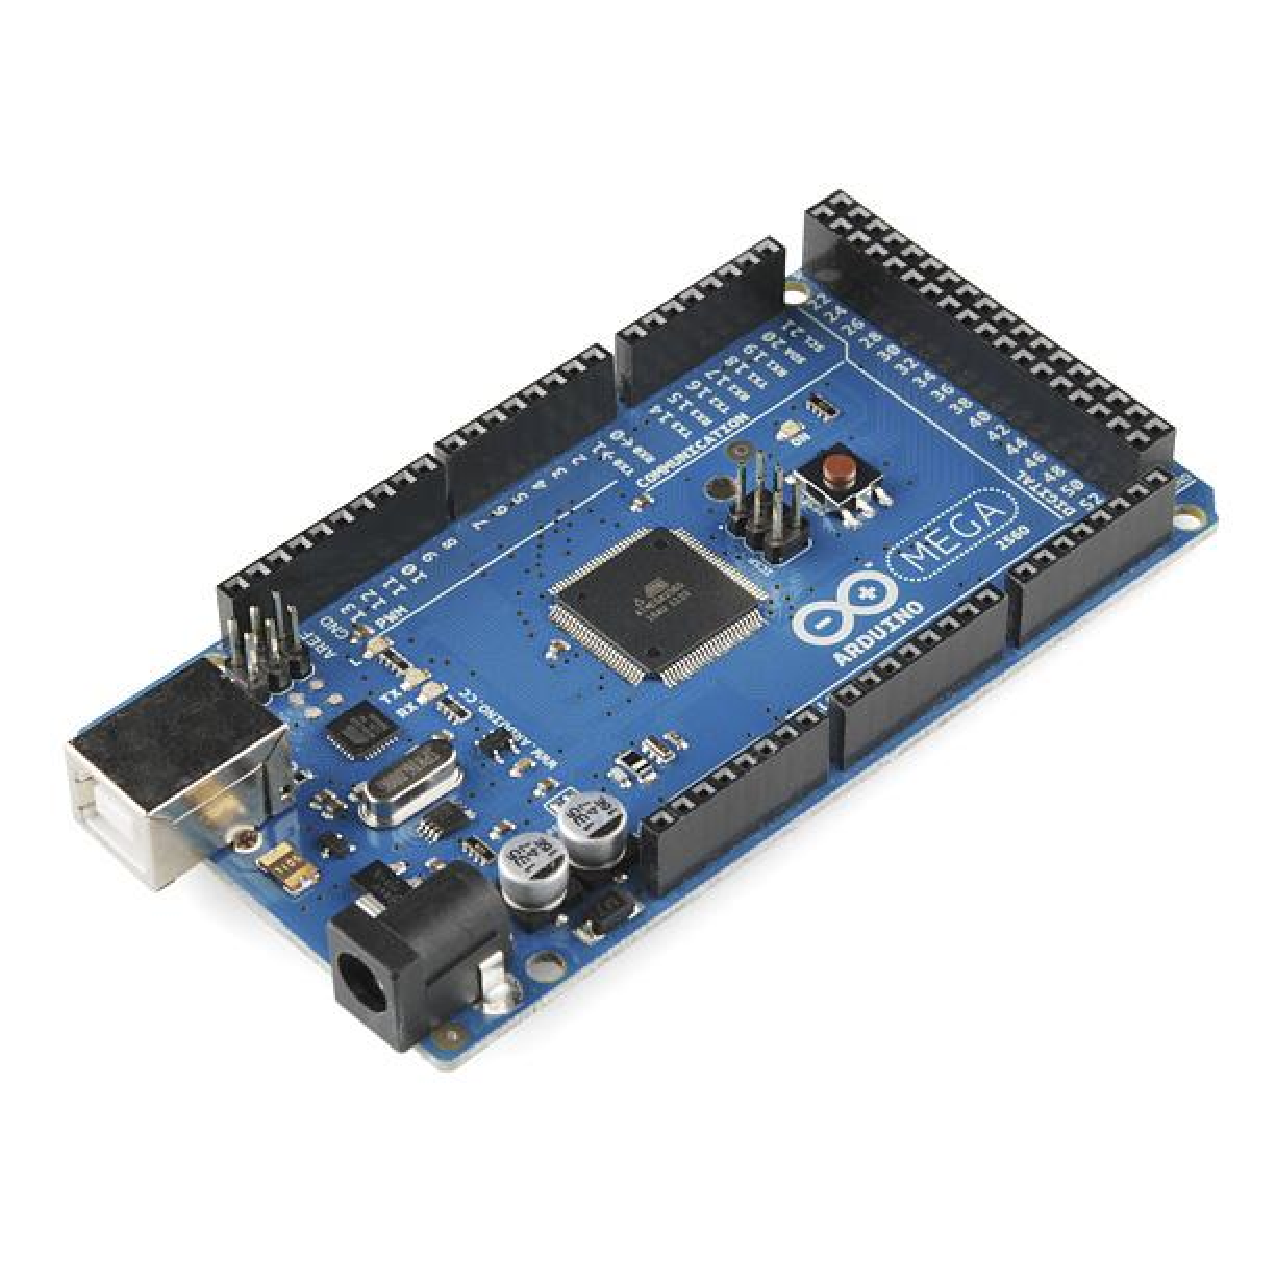
\includegraphics[width=.6\textwidth]{figuras/arduino.eps}
  \caption{\label{fig:arduino}Arduino Mega2560.}
  \end{center}
  \end{figure}
  % }}}

  A escolha da placa foi motivada por diversos fatores.
  Primeiramente, ela é capaz de realizar as demandas de controle do
  veículo, bem como possui um número de portas adequado. Além disso,
  é relativamente barata se comparada a outras plataformas de
  microcontroladores. Seu software é multiplataforma, proporcionando
  a interface com o Linux e possui um ambiente de programação simples,
  claro e bastante familiar.

% Fim da parte do PG }}}
